\section{Auswertung}
\label{sec:Auswertung}
Jegliche Fehlerrechnung wurde mit der Python-Bibliothek uncertainties \cite{uncertainties} absolviert. Trotz dessen sind die Formeln für
die Unsicherheiten in den jeweiligen Abschnitten angegeben. Allgemeine Rechnungen wurden mit der Python-Bilbiothek numpy \cite{numpy} automatisiert.
\subsection{Kennlinenschar einer Hochvakuumdiode}
In der Tabelle \ref{tab:charcurve} sind die gemessenen Absaugströme aufgetragen. Der letzte Eintrag von $I_{\text{A}1}$ ()
\begin{figure}
    \centering
    \caption{Kennlinienschar bei verschiedenen Heizleistungen}
    \label{fig:charcurve}
    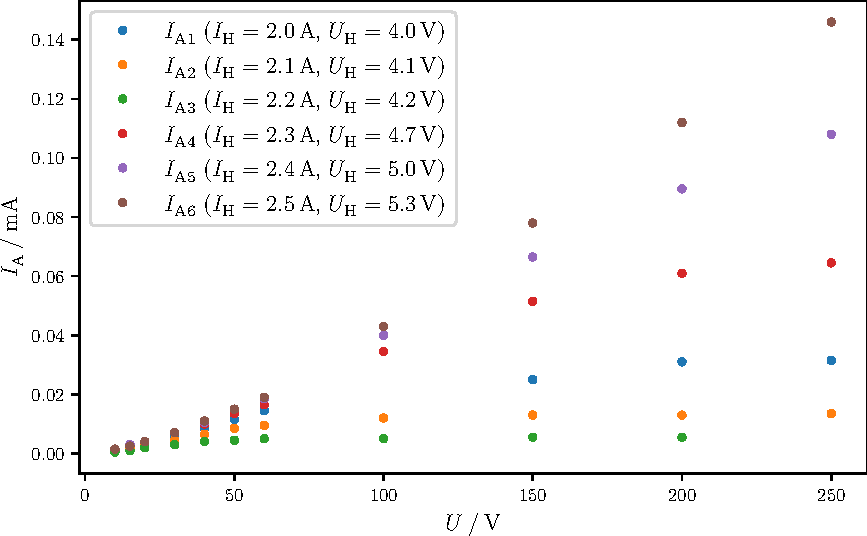
\includegraphics[width = \textwidth]{build/charcurve.pdf}
\end{figure}
\begin{table}
    \centering
    \caption{Berechnete Temperaturen und Austrittsarbeit}
    \label{tab:charcurve}
    \begin{tabular}{S[table-format = 3.0] S[table-format = 1.2] S[table-format = 1.2] S[table-format = 1.2] S[table-format = 1.2]
        S[table-format = 1.2] S[table-format = 1.2]}
        \toprule
        {$U_A \mathbin{/} \si{\volt}$} & {$I_{\text{A}1} \mathbin{/} \SI{20}{\milli\ampere}$} & {$I_{\text{A}2} \mathbin{/} \SI{20}{\milli\ampere}$} &
        {$I_{\text{A}3} \mathbin{/} \SI{20}{\milli\ampere}$} & {$I_{\text{A}4} \mathbin{/} \SI{20}{\milli\ampere}$} & 
        {$I_{\text{A}5} \mathbin{/} \SI{20}{\milli\ampere}$} & {$I_{\text{A}6} \mathbin{/} \SI{20}{\milli\ampere}$}
        \\
        \midrule
        10  & 0.01 & 0.02 & 0.02 & 0.03 & 0.03 & 0.03   \\
        15  & 0.02 & 0.04 & 0.04 & 0.05 & 0.06 & 0.05   \\
        20  & 0.04 & 0.05 & 0.06 & 0.08 & 0.08 & 0.08   \\
        30  & 0.06 & 0.09 & 0.11 & 0.14 & 0.14 & 0.14   \\
        40  & 0.08 & 0.13 & 0.17 & 0.2  & 0.21 & 0.22   \\
        50  & 0.09 & 0.17 & 0.23 & 0.27 & 0.3  & 0.3    \\
        60  & 0.1  & 0.19 & 0.29 & 0.33 & 0.37 & 0.38   \\
        100 & 0.1  & 0.24 & 0.24 & 0.69 & 0.8  & 0.86   \\
        150 & 0.11 & 0.26 & 0.5  & 1.03 & 1.33 & 1.56   \\
        200 & 0.11 & 0.26 & 0.62 & 1.22 & 1.79 & 2.24   \\
        250 & 0.0 & 0.27 & 0.63 & 1.29 & 2.16 & 2.92   \\
        \bottomrule
    \end{tabular}
\end{table}
In der Abbildung \ref{fig:charcurve} sind die Messwerte  der Absaugströme $I_{\text{A}1}$ bis $I_{\text{A}6}$ bei  6 verschiedenen Heizströmen ($I_\text{H}$)
bzw. -spannungen aufgetragen ($U_\text{H}$). 
Anhand der Graphik können die Sättigungsströme $I_\text{S}$für die Kennlinien von $I_{\text{A}1}$ bis $I_{\text{A}4}$ abgelesen werden.
Diese betragen in etwa
\begin{align*}
I_{\text{S}1} & = \SI{2.2}{\milli\ampere}   \\
I_{\text{S}2} & = \SI{5.4}{\milli\ampere}   \\
I_{\text{S}3} & = \SI{12.6}{\milli\ampere}  \\
I_{\text{S}4} & = \SI{25.8}{\milli\ampere}
\end{align*}
\subsection{Bestimmung des Raumladungsgebietes}
\begin{figure}
    \centering
    \caption{Regression zur Bestimmung des Raumladungsgebietes}
    \label{fig:exponent}
    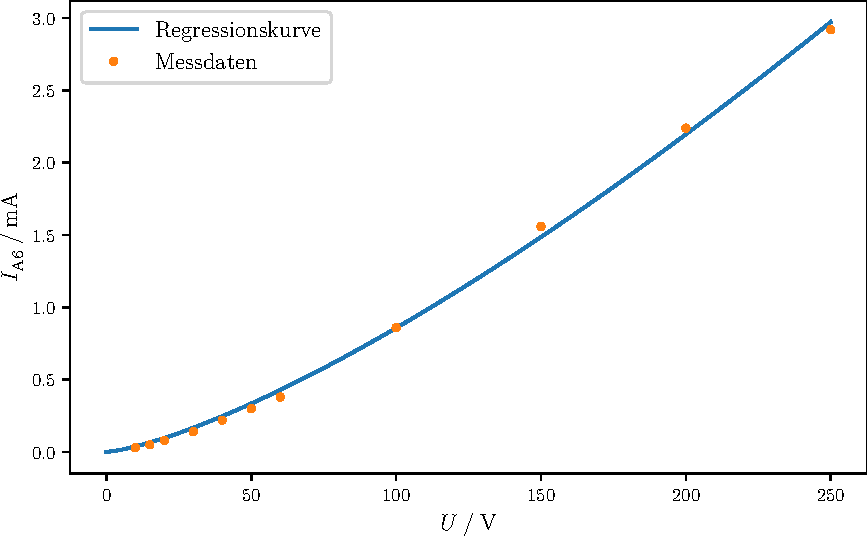
\includegraphics[width = \textwidth]{build/exponent.pdf}
\end{figure}
Zur Bestimmung des Raumladungsgebietes wird die Gültigkeit des Exponenten der Gleichung $REFERENZ$ an den Messwerten mittels Regression untersucht.
Dazu lässt sich die Regressionvorschrift als
\begin{equation}
    y = cV^d
\end{equation} 
schreiben.
Nach Durchführung der Regression und Anpassung der Spannungsintervalle ergeben sich die Regressionsparameter zu
\begin{align*}
    c & = \num{0.0150(9)} \\ 
    d & = \num{1.5001(114)} \; \text{.}
\end{align*}
Aufgrund der Anpassung des Intervalls lässt sich sagen, dass die $V^\frac{3}{2}$-Proportionalität zwischen $\SI{0}{\volt}$ und $\SI{150}{\volt}$ 
und somit auch das Raumladungsgebiet wiederzufinden ist.
\subsection{Bestimmung der Kathodentemperatur}
\begin{figure}
    \centering
    \caption{Untersuchung des Anlaufstromgebietes}
    \label{fig:startcurr}
    \includegraphics[width = \textwidth]{build/startcurr.pdf}
\end{figure}
Zunnächst muss die Spannunng wegen des Spannungsabfalls an dem Nanoamperemeter korrigiert werden.
Dafür wird das Produkt aus der Anlaufspannung und dem Innenwiderstand von $R_j = \SI{1}{\mega\ohm}$ hinzuaddiert.
\begin{equation}
    U = U_H + I R_j \; \text{.}
\end{equation}
Zur Bestimmung der Temperatur wird mit Hilfe des Anlaufstroms eine lineare Regression durchgeführt. 
Die Gesetzmäßigkeit $REFERENZ$ wird hierfür logarithmiert.
\begin{equation}
    \ln \left ( I \right ) = \frac{-e_0}{kT} V + \ln \left (c \right )
\end{equation}
Diese Gleichung in Regressionsparameter überführt ergibt
\begin{equation}
    y = mV + a \; \text{.}
\end{equation}
Mittels Rechnung mit python lassen sich die Parameter zu 
\begin{align*}
    m &= \num{-7.9646(4316)} \\
    a &= \num{-14.0669(2392)}
\end{align*}
berechnen.
Mit Hilfe der Beziehung 
\begin{equation}
    m = -\frac{e_0}{kT} \iff T = -\frac{e_0}{km}
\end{equation}
kann die Temperatur zu 
\begin{equation*}
    T = \SI{1460(80)}{\kelvin} 
\end{equation*}
bestimmt werden.
Die beiden Ausreißer bei $U_H = \SI{0}{\volt}$ und $U_H = \SI{0.1}{\volt}$ wurden nicht in der Regressionrechnung beachtet, da die Abweichungen zu stark sind.
Die errechneten Austrttsarbeiten sind in der Tabelle \ref{tab:tempwork} aufgetragen. Die vier $0.0$ Einträge deuten auf fehlende Sättigungsströme hin.
\begin{table}
    \centering
    \caption{Berechnete Temperaturen und Austrittsarbeit}
    \label{tab:tempwork}
    \begin{tabular}{S[table-format = 1.1] S[table-format = 1.1] S[table-format = 4.2] S[table-format = 2.2] S[table-format = 1.2]}
        \toprule
        {$U_H \mathbin{/} \si{\volt}$} & {$I_H \mathbin{/} \si{\ampere}$} & {$T \mathbin{/} \si{\kelvin}$} & {$I_S \mathbin{/} \si{\milli\ampere}$}
        & {$e_0\phi \mathbin{/} \si{\electronvolt}$}\\
        \midrule
        4.00 & 2.00 & 1924.11 & 2.20 & 1.84      \\
        4.10 & 2.10 & 1964.72 & 5.40 & 1.73      \\
        4.20 & 2.20 & 2004.18 & 12.6 & 1.63    \\
        4.70 & 2.30 & 2093.49 & 25.8 & 1.58    \\
        5.00 & 2.40 & 2154.28 & 0.0  & 0.0     \\
        5.30 & 2.50 & 2213.04 & 0.0  & 0.0     \\
        \bottomrule
    \end{tabular}
\end{table}
Der Mittelwert der Austrttsarbeit ergibt sich zu 
\begin{equation*}
    \bar{e_0\phi} = \SI{1.6947(565)}{\electronvolt}
\end{equation*}
